% Seminar 16: Review
% Statistics of Financial Markets -- Bachelor's programme, Bucharest University of Economic Studies
% GENERATED by latex/build_seminar16.py -- edit the generator, not this file.
% Student version by default; the instructor version is the *_solutions.tex wrapper.
\makeatletter\@ifundefined{ifsolutions}{\expandafter\newif\csname ifsolutions\endcsname}{}\makeatother

\newcommand{\coursename}{Statistics of Financial Markets}
% Preambul comun SFM -- Statistica piețelor financiare / Statistics of Financial Markets (Beamer, 16:9)
% Același design ca MFM. Înainte de % Preambul comun SFM -- Statistica piețelor financiare / Statistics of Financial Markets (Beamer, 16:9)
% Același design ca MFM. Înainte de % Preambul comun SFM -- Statistica piețelor financiare / Statistics of Financial Markets (Beamer, 16:9)
% Același design ca MFM. Înainte de \input{../../latex/preamble} se definește
%   \newcommand{\coursename}{Statistics of Financial Markets}      (EN)
%   \newcommand{\coursename}{Statistica piețelor financiare}       (RO)  și  \def\sfmlang{ro}
% Fișierele .tex se află în EN/Courses, EN/Seminars, RO/Cursuri, RO/Seminarii (două niveluri sub rădăcină).
% Deck-urile sînt generate de latex/build_chapterN.py / build_seminarN.py (vezi latex/sfm_build.py).

\documentclass[9pt, aspectratio=169, t]{beamer}
\providecommand{\coursename}{Statistics of Financial Markets}

% Ensure content fits on slides
\setbeamersize{text margin left=8mm, text margin right=8mm}

%=============================================================================
% THEME AND STYLE CONFIGURATION
%=============================================================================
\usetheme{default}
% Using default theme for clean header/footer control

% Color Palette (matching Redispatch PDF)
\definecolor{MainBlue}{RGB}{26, 58, 110}
\definecolor{AccentBlue}{RGB}{26, 58, 110}
\definecolor{IDAred}{RGB}{205, 0, 0}
\definecolor{DarkGray}{RGB}{51, 51, 51}
\definecolor{MediumGray}{RGB}{128, 128, 128}
\definecolor{LightGray}{RGB}{248, 248, 248}
\definecolor{VeryLightGray}{RGB}{235, 235, 235}
\definecolor{KeynoteGray}{RGB}{218, 218, 218}
\definecolor{SectionGray}{RGB}{120, 120, 120}
\definecolor{FooterGray}{RGB}{100, 100, 100}
\definecolor{Crimson}{RGB}{220, 53, 69}
\definecolor{Forest}{RGB}{46, 125, 50}
\definecolor{Amber}{RGB}{181, 133, 63}
\definecolor{Orange}{RGB}{230, 126, 34}
\definecolor{Purple}{RGB}{142, 68, 173}

% Gradient background (exact Keynote 315° gradient: white to RGB 218,218,218)
\setbeamertemplate{background}{%
    \begin{tikzpicture}[remember picture, overlay]
        \shade[shading=axis, shading angle=315,
        top color=white, bottom color=KeynoteGray]
        (current page.south west) rectangle (current page.north east);
    \end{tikzpicture}%
}
% Fallback solid color for compatibility
\setbeamercolor{background canvas}{bg=}

\setbeamercolor{palette primary}{bg=MainBlue, fg=white}
\setbeamercolor{palette secondary}{bg=MainBlue!85, fg=white}
\setbeamercolor{palette tertiary}{bg=MainBlue!70, fg=white}
\setbeamercolor{structure}{fg=MainBlue}
\setbeamercolor{title}{fg=IDAred}
\setbeamercolor{frametitle}{fg=IDAred, bg=}
\setbeamercolor{block title}{bg=MainBlue, fg=white}
\setbeamercolor{block body}{bg=VeryLightGray, fg=DarkGray}
\setbeamercolor{block title alerted}{bg=Crimson, fg=white}
\setbeamercolor{block body alerted}{bg=Crimson!8, fg=DarkGray}
\setbeamercolor{block title example}{bg=Forest, fg=white}
\setbeamercolor{block body example}{bg=Forest!8, fg=DarkGray}
\setbeamercolor{item}{fg=MainBlue}

% Footer colors (override Madrid theme blue)
\setbeamercolor{author in head/foot}{fg=FooterGray, bg=}
\setbeamercolor{title in head/foot}{fg=FooterGray, bg=}
\setbeamercolor{date in head/foot}{fg=FooterGray, bg=}
\setbeamercolor{section in head/foot}{fg=FooterGray, bg=}
\setbeamercolor{subsection in head/foot}{fg=FooterGray, bg=}

% Bullet styles (apply everywhere including blocks)
\setbeamertemplate{itemize item}{\color{MainBlue}$\boxdot$}
\setbeamertemplate{itemize subitem}{\color{MainBlue}$\blacktriangleright$}
\setbeamertemplate{itemize subsubitem}{\color{MainBlue}\tiny$\bullet$}
\setbeamertemplate{itemize/enumerate body begin}{\normalsize}
\setbeamertemplate{itemize/enumerate subbody begin}{\normalsize}

% Item spacing - compact style
\setlength{\leftmargini}{10pt}       % Level 1: minimal indent
\setlength{\leftmarginii}{10pt}      % Level 2: minimal additional indent
% Compact list spacing (zero extra space before/after lists in blocks)
\makeatletter
\def\@listi{\leftmargin\leftmargini \topsep 0pt \parsep 0pt \itemsep 0pt}
\def\@listii{\leftmargin\leftmarginii \topsep 0pt \parsep 0pt \itemsep 0pt}
\makeatother

\setbeamertemplate{navigation symbols}{}

%=============================================================================
% CUSTOM HEADLINE
%=============================================================================
\setbeamertemplate{headline}{%
    \vskip10pt%
    \hbox to \paperwidth{%
        \hskip0.5cm%
        {\small\color{FooterGray}\renewcommand{\hyperlink}[2]{##2}\insertsectionhead}%
        \hfill%
        \textcolor{FooterGray}{\small\insertframenumber}%
        \hskip0.5cm%
    }%
    \vskip4pt%
    {\color{FooterGray}\hrule height 0.4pt}%
}

%=============================================================================
% CUSTOM FOOTER
%=============================================================================
\usepackage{fontawesome5}

\setbeamertemplate{footline}{%
    {\color{FooterGray}\hrule height 0.4pt}%
    \vskip4pt%
    \hbox to \paperwidth{%
        \hskip0.5cm%
        \textcolor{FooterGray}{\small\coursename}%
        \hfill%
        \raisebox{-0.1em}{%
            \begin{tikzpicture}[x=0.08em, y=0.08em, line width=0.4pt]
                \draw[FooterGray] (0,3) -- (1,4) -- (2,3.5) -- (3,5) -- (4,4) -- (5,6) -- (6,5.5) -- (7,4) -- (8,5) -- (9,7) -- (10,6) -- (11,5) -- (12,6.5) -- (13,8) -- (14,7) -- (15,6) -- (16,7.5) -- (17,9) -- (18,8) -- (19,7) -- (20,8.5) -- (21,10) -- (22,9) -- (23,8) -- (24,9.5);
            \end{tikzpicture}%
        }%
        \hskip0.5cm%
    }%
    \vskip6pt%
}

%=============================================================================
% PACKAGES
%=============================================================================
\usepackage[utf8]{inputenc}
\DeclareUnicodeCharacter{03B1}{\ensuremath{\alpha}}
\usepackage[T1]{fontenc}
\usepackage{amsmath, amssymb, amsthm}
\usepackage{mathtools}
\usepackage{bm}
\usepackage{tikz}
\usetikzlibrary{arrows.meta, positioning, shapes, calc, decorations.pathreplacing, shadings}
\usepackage{booktabs}
\usepackage{multirow}
\usepackage{array}
\usepackage{graphicx}
\usepackage{hyperref}
\usepackage{colortbl}
\usepackage{listings}
\lstset{language=Python, basicstyle=\ttfamily\scriptsize, keywordstyle=\color{MainBlue}\bfseries,
  commentstyle=\color{Forest}, stringstyle=\color{Crimson}, breaklines=true,
  frame=none, backgroundcolor=\color{VeryLightGray}, xleftmargin=2mm}
\hypersetup{colorlinks=true, linkcolor=MainBlue, urlcolor=MainBlue}
\graphicspath{{../../logos/}{../../charts/}{../../photos/}}
\usepackage{xcolor}
\hfuzz=2pt  % Suppress tiny overfull warnings (<2pt)
\vfuzz=2pt  % Suppress tiny vertical overfull warnings (<2pt)

%=============================================================================
% QUANTLET COMMANDS
%   \quantlet{<displayed name>}{<url>}       (generic, compatible with the older SFM decks)
%   \sfmquantlet{Ch_05}{SFM_ch5_garch}       -> https://github.com/danpele/SFM/tree/main/Quantlets/Ch_05/SFM_ch5_garch
%   \qlurl{<folder>} is defined per chapter by the generator (Quantlets/Ch_NN/<folder>)
%=============================================================================
\newcommand{\sfmrepo}{https://github.com/danpele/SFM}
\newcommand{\sfmqlbase}{https://github.com/danpele/SFM/tree/main/Quantlets}
\newcommand{\quantlet}[2]{%
    \hfill\href{#2}{%
        \raisebox{-0.15em}{
\includegraphics[height=0.7em]{ql_logo.png}}%
        \textcolor{MainBlue}{\tiny\ #1}%
    }%
}
\newcommand{\sfmquantlet}[2]{\quantlet{\detokenize{#2}}{\sfmqlbase/#1/#2}}

%=============================================================================
% NOTEBOOKS (Google Colab)
%   \colaburl{notebooks/EN/chapter5_seminar_notebook.ipynb} -> the Colab link of a file in the SFM repo
%   \nb: the chapter notebook (each seminar deck redefines it with \renewcommand)
%=============================================================================
\newcommand{\colaburl}[1]{https://colab.research.google.com/github/danpele/SFM/blob/main/#1}
\newcommand{\nb}{https://colab.research.google.com/github/danpele/SFM/tree/main/notebooks/EN}
\newcommand{\nbname}{notebooks/EN}

%=============================================================================
% SLIDE HELPERS (used by the generators; the same as in MFM)
%=============================================================================
% local font size for list bodies (the preamble forces \normalsize)
\newcommand{\itemsize}[1]{\setbeamertemplate{itemize/enumerate body begin}{#1}\setbeamertemplate{itemize/enumerate subbody begin}{#1}}
\newcommand{\intitle}[1]{{\hypersetup{urlcolor=white}#1}}   % white links inside coloured title bars
\newcommand{\imgcap}[1]{{\scriptsize #1}\\[0.5mm]}          % caption under a photo
\newcommand{\imgcredit}[2]{{\tiny\color{FooterGray}\href{#1}{#2}}}   % image credit: source URL, author/licence
\newcommand{\aiprompt}[1]{{\ttfamily\color{MainBlue}#1}}     % a prompt to an AI assistant

%=============================================================================
% SEMINARS: student version by default; the instructor wrapper *_solutions.tex sets \solutionstrue
%=============================================================================
\makeatletter\@ifundefined{ifsolutions}{\expandafter\newif\csname ifsolutions\endcsname}{}\makeatother
\newcommand{\solonly}[1]{\ifsolutions #1\fi}
\newcommand{\propsub}{\ifsolutions\else\framesubtitle{\ifdefined\sfmlang Rezolvarea se discută la seminar\else Solution discussed in class\fi}\fi}

%=============================================================================
% APPENDIX AND CHAPTER LINKS (latex/appendix_links.py writes the calls; it also re-declares these
% macros before \begin{document}, so the decks compile with or without this preamble block)
%=============================================================================
\providecommand{\sfmapplink}[3]{\hypertarget{#2}{}\hyperlink{#1}{\beamergotobutton{#3}}}
\providecommand{\sfmappback}[2]{\begin{tikzpicture}[remember picture,overlay]\node[anchor=south east] at ([xshift=-3mm,yshift=7mm]current page.south east){\hyperlink{#1}{\beamerreturnbutton{#2}}};\end{tikzpicture}}
\providecommand{\sfmchlink}[2]{\href{#1}{#2}}
\providecommand{\sfmchlinkt}[2]{\href{#1}{\usebeamercolor[fg]{frametitle}#2}}

%=============================================================================
% QUANTINAR COMMAND: link către un curs Quantinar (subiecte avansate)
%=============================================================================
\newcommand{\quantinar}[2]{%
    \href{#2}{%
        \raisebox{-0.15em}{
\includegraphics[height=0.8em]{qr_logo.png}}%
        \textcolor{MainBlue}{\scriptsize\ #1}%
    }%
}

%=============================================================================
% CUSTOM TITLE PAGE
%=============================================================================
\defbeamertemplate*{title page}{hybrid}[1][]
{
    \vspace{0.2cm}
    % Logos row - top header (with clickable links)
    \begin{center}
        \href{https://www.ase.ro}{
\includegraphics[height=1.0cm]{ase_logo.png}}\hspace{0.3cm}%
        \href{https://theida.net}{
\includegraphics[height=1.0cm]{ida_logo.png}}\hspace{0.3cm}%
        \href{https://blockchain-research-center.com}{
\includegraphics[height=1.0cm]{brc_logo.png}}\hspace{0.3cm}%
        \href{https://www.ai4efin.ase.ro}{
\includegraphics[height=1.0cm]{ai4efin_logo.png}}\hspace{0.3cm}%
        \href{https://ipe.ro/new}{
\includegraphics[height=1.0cm]{acad_logo.png}}\hspace{0.3cm}%
        \href{https://www.digital-finance-msca.com}{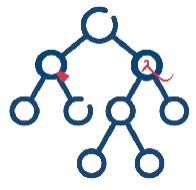
\includegraphics[height=1.0cm]{msca_logo.png}}%
    \end{center}

    \vspace{0.6cm}

    % Main title with Q logos on sides (with clickable links)
    \begin{center}
        \begin{minipage}{0.1\textwidth}
            \centering
            \href{https://quantlet.com}{
\includegraphics[height=1.1cm]{ql_logo.png}}
        \end{minipage}%
        \begin{minipage}{0.78\textwidth}
            \centering
            {\LARGE\bfseries\usebeamercolor[fg]{title}\inserttitle}

            \vspace{0.3cm}

            {\usebeamerfont{subtitle}\usebeamercolor[fg]{title}\insertsubtitle}
        \end{minipage}%
        \begin{minipage}{0.1\textwidth}
            \centering
            \href{https://quantinar.com}{
\includegraphics[height=1.1cm]{qr_logo.png}}
        \end{minipage}
    \end{center}

    \vspace{0.6cm}

    % Authors (left aligned)
    \hspace{0.5cm}{\usebeamerfont{author}\insertauthor}

    \vspace{0.3cm}

    % Institute/Affiliations (left aligned)
    \hspace{0.5cm}\begin{minipage}[t]{0.9\textwidth}
        \raggedright\small\insertinstitute
    \end{minipage}
}

%=============================================================================
% THEOREM ENVIRONMENTS
%=============================================================================
\theoremstyle{definition}
\setbeamertemplate{theorems}[numbered]
\ifdefined\sfmlang
\newtheorem{defn}{Definiție}
\newtheorem{thm}{Teoremă}
\newtheorem{prop}{Propoziție}
\newtheorem{rmk}{Observație}
\else
\newtheorem{defn}{Definition}
\newtheorem{thm}{Theorem}
\newtheorem{prop}{Proposition}
\newtheorem{rmk}{Remark}
\fi

%=============================================================================
% CENTRED MINIPAGE (no extra vertical space)
%=============================================================================
\newenvironment{cminipage}[1]{%
    \par\noindent\hfill\begin{minipage}{#1}\ignorespaces
}{%
    \end{minipage}\hfill\null\par
}

%=============================================================================
% CUSTOM COMMANDS
%=============================================================================
\newcommand{\E}{\mathbb{E}}
\newcommand{\Var}{\text{Var}}
\newcommand{\Cov}{\text{Cov}}
\newcommand{\Corr}{\text{Corr}}
\newcommand{\R}{\mathbb{R}}
\newcommand{\N}{\mathbb{N}}
\newcommand{\Z}{\mathbb{Z}}
\newcommand{\B}{\mathbf{B}}
\newcommand{\imark}{\textcolor{MainBlue}{\textbullet}}
\newcommand{\RMSE}{\text{RMSE}}
\newcommand{\MAE}{\text{MAE}}
\newcommand{\MAPE}{\text{MAPE}}

 se definește
%   \newcommand{\coursename}{Statistics of Financial Markets}      (EN)
%   \newcommand{\coursename}{Statistica piețelor financiare}       (RO)  și  \def\sfmlang{ro}
% Fișierele .tex se află în EN/Courses, EN/Seminars, RO/Cursuri, RO/Seminarii (două niveluri sub rădăcină).
% Deck-urile sînt generate de latex/build_chapterN.py / build_seminarN.py (vezi latex/sfm_build.py).

\documentclass[9pt, aspectratio=169, t]{beamer}
\providecommand{\coursename}{Statistics of Financial Markets}

% Ensure content fits on slides
\setbeamersize{text margin left=8mm, text margin right=8mm}

%=============================================================================
% THEME AND STYLE CONFIGURATION
%=============================================================================
\usetheme{default}
% Using default theme for clean header/footer control

% Color Palette (matching Redispatch PDF)
\definecolor{MainBlue}{RGB}{26, 58, 110}
\definecolor{AccentBlue}{RGB}{26, 58, 110}
\definecolor{IDAred}{RGB}{205, 0, 0}
\definecolor{DarkGray}{RGB}{51, 51, 51}
\definecolor{MediumGray}{RGB}{128, 128, 128}
\definecolor{LightGray}{RGB}{248, 248, 248}
\definecolor{VeryLightGray}{RGB}{235, 235, 235}
\definecolor{KeynoteGray}{RGB}{218, 218, 218}
\definecolor{SectionGray}{RGB}{120, 120, 120}
\definecolor{FooterGray}{RGB}{100, 100, 100}
\definecolor{Crimson}{RGB}{220, 53, 69}
\definecolor{Forest}{RGB}{46, 125, 50}
\definecolor{Amber}{RGB}{181, 133, 63}
\definecolor{Orange}{RGB}{230, 126, 34}
\definecolor{Purple}{RGB}{142, 68, 173}

% Gradient background (exact Keynote 315° gradient: white to RGB 218,218,218)
\setbeamertemplate{background}{%
    \begin{tikzpicture}[remember picture, overlay]
        \shade[shading=axis, shading angle=315,
        top color=white, bottom color=KeynoteGray]
        (current page.south west) rectangle (current page.north east);
    \end{tikzpicture}%
}
% Fallback solid color for compatibility
\setbeamercolor{background canvas}{bg=}

\setbeamercolor{palette primary}{bg=MainBlue, fg=white}
\setbeamercolor{palette secondary}{bg=MainBlue!85, fg=white}
\setbeamercolor{palette tertiary}{bg=MainBlue!70, fg=white}
\setbeamercolor{structure}{fg=MainBlue}
\setbeamercolor{title}{fg=IDAred}
\setbeamercolor{frametitle}{fg=IDAred, bg=}
\setbeamercolor{block title}{bg=MainBlue, fg=white}
\setbeamercolor{block body}{bg=VeryLightGray, fg=DarkGray}
\setbeamercolor{block title alerted}{bg=Crimson, fg=white}
\setbeamercolor{block body alerted}{bg=Crimson!8, fg=DarkGray}
\setbeamercolor{block title example}{bg=Forest, fg=white}
\setbeamercolor{block body example}{bg=Forest!8, fg=DarkGray}
\setbeamercolor{item}{fg=MainBlue}

% Footer colors (override Madrid theme blue)
\setbeamercolor{author in head/foot}{fg=FooterGray, bg=}
\setbeamercolor{title in head/foot}{fg=FooterGray, bg=}
\setbeamercolor{date in head/foot}{fg=FooterGray, bg=}
\setbeamercolor{section in head/foot}{fg=FooterGray, bg=}
\setbeamercolor{subsection in head/foot}{fg=FooterGray, bg=}

% Bullet styles (apply everywhere including blocks)
\setbeamertemplate{itemize item}{\color{MainBlue}$\boxdot$}
\setbeamertemplate{itemize subitem}{\color{MainBlue}$\blacktriangleright$}
\setbeamertemplate{itemize subsubitem}{\color{MainBlue}\tiny$\bullet$}
\setbeamertemplate{itemize/enumerate body begin}{\normalsize}
\setbeamertemplate{itemize/enumerate subbody begin}{\normalsize}

% Item spacing - compact style
\setlength{\leftmargini}{10pt}       % Level 1: minimal indent
\setlength{\leftmarginii}{10pt}      % Level 2: minimal additional indent
% Compact list spacing (zero extra space before/after lists in blocks)
\makeatletter
\def\@listi{\leftmargin\leftmargini \topsep 0pt \parsep 0pt \itemsep 0pt}
\def\@listii{\leftmargin\leftmarginii \topsep 0pt \parsep 0pt \itemsep 0pt}
\makeatother

\setbeamertemplate{navigation symbols}{}

%=============================================================================
% CUSTOM HEADLINE
%=============================================================================
\setbeamertemplate{headline}{%
    \vskip10pt%
    \hbox to \paperwidth{%
        \hskip0.5cm%
        {\small\color{FooterGray}\renewcommand{\hyperlink}[2]{##2}\insertsectionhead}%
        \hfill%
        \textcolor{FooterGray}{\small\insertframenumber}%
        \hskip0.5cm%
    }%
    \vskip4pt%
    {\color{FooterGray}\hrule height 0.4pt}%
}

%=============================================================================
% CUSTOM FOOTER
%=============================================================================
\usepackage{fontawesome5}

\setbeamertemplate{footline}{%
    {\color{FooterGray}\hrule height 0.4pt}%
    \vskip4pt%
    \hbox to \paperwidth{%
        \hskip0.5cm%
        \textcolor{FooterGray}{\small\coursename}%
        \hfill%
        \raisebox{-0.1em}{%
            \begin{tikzpicture}[x=0.08em, y=0.08em, line width=0.4pt]
                \draw[FooterGray] (0,3) -- (1,4) -- (2,3.5) -- (3,5) -- (4,4) -- (5,6) -- (6,5.5) -- (7,4) -- (8,5) -- (9,7) -- (10,6) -- (11,5) -- (12,6.5) -- (13,8) -- (14,7) -- (15,6) -- (16,7.5) -- (17,9) -- (18,8) -- (19,7) -- (20,8.5) -- (21,10) -- (22,9) -- (23,8) -- (24,9.5);
            \end{tikzpicture}%
        }%
        \hskip0.5cm%
    }%
    \vskip6pt%
}

%=============================================================================
% PACKAGES
%=============================================================================
\usepackage[utf8]{inputenc}
\DeclareUnicodeCharacter{03B1}{\ensuremath{\alpha}}
\usepackage[T1]{fontenc}
\usepackage{amsmath, amssymb, amsthm}
\usepackage{mathtools}
\usepackage{bm}
\usepackage{tikz}
\usetikzlibrary{arrows.meta, positioning, shapes, calc, decorations.pathreplacing, shadings}
\usepackage{booktabs}
\usepackage{multirow}
\usepackage{array}
\usepackage{graphicx}
\usepackage{hyperref}
\usepackage{colortbl}
\usepackage{listings}
\lstset{language=Python, basicstyle=\ttfamily\scriptsize, keywordstyle=\color{MainBlue}\bfseries,
  commentstyle=\color{Forest}, stringstyle=\color{Crimson}, breaklines=true,
  frame=none, backgroundcolor=\color{VeryLightGray}, xleftmargin=2mm}
\hypersetup{colorlinks=true, linkcolor=MainBlue, urlcolor=MainBlue}
\graphicspath{{../../logos/}{../../charts/}{../../photos/}}
\usepackage{xcolor}
\hfuzz=2pt  % Suppress tiny overfull warnings (<2pt)
\vfuzz=2pt  % Suppress tiny vertical overfull warnings (<2pt)

%=============================================================================
% QUANTLET COMMANDS
%   \quantlet{<displayed name>}{<url>}       (generic, compatible with the older SFM decks)
%   \sfmquantlet{Ch_05}{SFM_ch5_garch}       -> https://github.com/danpele/SFM/tree/main/Quantlets/Ch_05/SFM_ch5_garch
%   \qlurl{<folder>} is defined per chapter by the generator (Quantlets/Ch_NN/<folder>)
%=============================================================================
\newcommand{\sfmrepo}{https://github.com/danpele/SFM}
\newcommand{\sfmqlbase}{https://github.com/danpele/SFM/tree/main/Quantlets}
\newcommand{\quantlet}[2]{%
    \hfill\href{#2}{%
        \raisebox{-0.15em}{
\includegraphics[height=0.7em]{ql_logo.png}}%
        \textcolor{MainBlue}{\tiny\ #1}%
    }%
}
\newcommand{\sfmquantlet}[2]{\quantlet{\detokenize{#2}}{\sfmqlbase/#1/#2}}

%=============================================================================
% NOTEBOOKS (Google Colab)
%   \colaburl{notebooks/EN/chapter5_seminar_notebook.ipynb} -> the Colab link of a file in the SFM repo
%   \nb: the chapter notebook (each seminar deck redefines it with \renewcommand)
%=============================================================================
\newcommand{\colaburl}[1]{https://colab.research.google.com/github/danpele/SFM/blob/main/#1}
\newcommand{\nb}{https://colab.research.google.com/github/danpele/SFM/tree/main/notebooks/EN}
\newcommand{\nbname}{notebooks/EN}

%=============================================================================
% SLIDE HELPERS (used by the generators; the same as in MFM)
%=============================================================================
% local font size for list bodies (the preamble forces \normalsize)
\newcommand{\itemsize}[1]{\setbeamertemplate{itemize/enumerate body begin}{#1}\setbeamertemplate{itemize/enumerate subbody begin}{#1}}
\newcommand{\intitle}[1]{{\hypersetup{urlcolor=white}#1}}   % white links inside coloured title bars
\newcommand{\imgcap}[1]{{\scriptsize #1}\\[0.5mm]}          % caption under a photo
\newcommand{\imgcredit}[2]{{\tiny\color{FooterGray}\href{#1}{#2}}}   % image credit: source URL, author/licence
\newcommand{\aiprompt}[1]{{\ttfamily\color{MainBlue}#1}}     % a prompt to an AI assistant

%=============================================================================
% SEMINARS: student version by default; the instructor wrapper *_solutions.tex sets \solutionstrue
%=============================================================================
\makeatletter\@ifundefined{ifsolutions}{\expandafter\newif\csname ifsolutions\endcsname}{}\makeatother
\newcommand{\solonly}[1]{\ifsolutions #1\fi}
\newcommand{\propsub}{\ifsolutions\else\framesubtitle{\ifdefined\sfmlang Rezolvarea se discută la seminar\else Solution discussed in class\fi}\fi}

%=============================================================================
% APPENDIX AND CHAPTER LINKS (latex/appendix_links.py writes the calls; it also re-declares these
% macros before \begin{document}, so the decks compile with or without this preamble block)
%=============================================================================
\providecommand{\sfmapplink}[3]{\hypertarget{#2}{}\hyperlink{#1}{\beamergotobutton{#3}}}
\providecommand{\sfmappback}[2]{\begin{tikzpicture}[remember picture,overlay]\node[anchor=south east] at ([xshift=-3mm,yshift=7mm]current page.south east){\hyperlink{#1}{\beamerreturnbutton{#2}}};\end{tikzpicture}}
\providecommand{\sfmchlink}[2]{\href{#1}{#2}}
\providecommand{\sfmchlinkt}[2]{\href{#1}{\usebeamercolor[fg]{frametitle}#2}}

%=============================================================================
% QUANTINAR COMMAND: link către un curs Quantinar (subiecte avansate)
%=============================================================================
\newcommand{\quantinar}[2]{%
    \href{#2}{%
        \raisebox{-0.15em}{
\includegraphics[height=0.8em]{qr_logo.png}}%
        \textcolor{MainBlue}{\scriptsize\ #1}%
    }%
}

%=============================================================================
% CUSTOM TITLE PAGE
%=============================================================================
\defbeamertemplate*{title page}{hybrid}[1][]
{
    \vspace{0.2cm}
    % Logos row - top header (with clickable links)
    \begin{center}
        \href{https://www.ase.ro}{
\includegraphics[height=1.0cm]{ase_logo.png}}\hspace{0.3cm}%
        \href{https://theida.net}{
\includegraphics[height=1.0cm]{ida_logo.png}}\hspace{0.3cm}%
        \href{https://blockchain-research-center.com}{
\includegraphics[height=1.0cm]{brc_logo.png}}\hspace{0.3cm}%
        \href{https://www.ai4efin.ase.ro}{
\includegraphics[height=1.0cm]{ai4efin_logo.png}}\hspace{0.3cm}%
        \href{https://ipe.ro/new}{
\includegraphics[height=1.0cm]{acad_logo.png}}\hspace{0.3cm}%
        \href{https://www.digital-finance-msca.com}{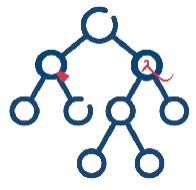
\includegraphics[height=1.0cm]{msca_logo.png}}%
    \end{center}

    \vspace{0.6cm}

    % Main title with Q logos on sides (with clickable links)
    \begin{center}
        \begin{minipage}{0.1\textwidth}
            \centering
            \href{https://quantlet.com}{
\includegraphics[height=1.1cm]{ql_logo.png}}
        \end{minipage}%
        \begin{minipage}{0.78\textwidth}
            \centering
            {\LARGE\bfseries\usebeamercolor[fg]{title}\inserttitle}

            \vspace{0.3cm}

            {\usebeamerfont{subtitle}\usebeamercolor[fg]{title}\insertsubtitle}
        \end{minipage}%
        \begin{minipage}{0.1\textwidth}
            \centering
            \href{https://quantinar.com}{
\includegraphics[height=1.1cm]{qr_logo.png}}
        \end{minipage}
    \end{center}

    \vspace{0.6cm}

    % Authors (left aligned)
    \hspace{0.5cm}{\usebeamerfont{author}\insertauthor}

    \vspace{0.3cm}

    % Institute/Affiliations (left aligned)
    \hspace{0.5cm}\begin{minipage}[t]{0.9\textwidth}
        \raggedright\small\insertinstitute
    \end{minipage}
}

%=============================================================================
% THEOREM ENVIRONMENTS
%=============================================================================
\theoremstyle{definition}
\setbeamertemplate{theorems}[numbered]
\ifdefined\sfmlang
\newtheorem{defn}{Definiție}
\newtheorem{thm}{Teoremă}
\newtheorem{prop}{Propoziție}
\newtheorem{rmk}{Observație}
\else
\newtheorem{defn}{Definition}
\newtheorem{thm}{Theorem}
\newtheorem{prop}{Proposition}
\newtheorem{rmk}{Remark}
\fi

%=============================================================================
% CENTRED MINIPAGE (no extra vertical space)
%=============================================================================
\newenvironment{cminipage}[1]{%
    \par\noindent\hfill\begin{minipage}{#1}\ignorespaces
}{%
    \end{minipage}\hfill\null\par
}

%=============================================================================
% CUSTOM COMMANDS
%=============================================================================
\newcommand{\E}{\mathbb{E}}
\newcommand{\Var}{\text{Var}}
\newcommand{\Cov}{\text{Cov}}
\newcommand{\Corr}{\text{Corr}}
\newcommand{\R}{\mathbb{R}}
\newcommand{\N}{\mathbb{N}}
\newcommand{\Z}{\mathbb{Z}}
\newcommand{\B}{\mathbf{B}}
\newcommand{\imark}{\textcolor{MainBlue}{\textbullet}}
\newcommand{\RMSE}{\text{RMSE}}
\newcommand{\MAE}{\text{MAE}}
\newcommand{\MAPE}{\text{MAPE}}

 se definește
%   \newcommand{\coursename}{Statistics of Financial Markets}      (EN)
%   \newcommand{\coursename}{Statistica piețelor financiare}       (RO)  și  \def\sfmlang{ro}
% Fișierele .tex se află în EN/Courses, EN/Seminars, RO/Cursuri, RO/Seminarii (două niveluri sub rădăcină).
% Deck-urile sînt generate de latex/build_chapterN.py / build_seminarN.py (vezi latex/sfm_build.py).

\documentclass[9pt, aspectratio=169, t]{beamer}
\providecommand{\coursename}{Statistics of Financial Markets}

% Ensure content fits on slides
\setbeamersize{text margin left=8mm, text margin right=8mm}

%=============================================================================
% THEME AND STYLE CONFIGURATION
%=============================================================================
\usetheme{default}
% Using default theme for clean header/footer control

% Color Palette (matching Redispatch PDF)
\definecolor{MainBlue}{RGB}{26, 58, 110}
\definecolor{AccentBlue}{RGB}{26, 58, 110}
\definecolor{IDAred}{RGB}{205, 0, 0}
\definecolor{DarkGray}{RGB}{51, 51, 51}
\definecolor{MediumGray}{RGB}{128, 128, 128}
\definecolor{LightGray}{RGB}{248, 248, 248}
\definecolor{VeryLightGray}{RGB}{235, 235, 235}
\definecolor{KeynoteGray}{RGB}{218, 218, 218}
\definecolor{SectionGray}{RGB}{120, 120, 120}
\definecolor{FooterGray}{RGB}{100, 100, 100}
\definecolor{Crimson}{RGB}{220, 53, 69}
\definecolor{Forest}{RGB}{46, 125, 50}
\definecolor{Amber}{RGB}{181, 133, 63}
\definecolor{Orange}{RGB}{230, 126, 34}
\definecolor{Purple}{RGB}{142, 68, 173}

% Gradient background (exact Keynote 315° gradient: white to RGB 218,218,218)
\setbeamertemplate{background}{%
    \begin{tikzpicture}[remember picture, overlay]
        \shade[shading=axis, shading angle=315,
        top color=white, bottom color=KeynoteGray]
        (current page.south west) rectangle (current page.north east);
    \end{tikzpicture}%
}
% Fallback solid color for compatibility
\setbeamercolor{background canvas}{bg=}

\setbeamercolor{palette primary}{bg=MainBlue, fg=white}
\setbeamercolor{palette secondary}{bg=MainBlue!85, fg=white}
\setbeamercolor{palette tertiary}{bg=MainBlue!70, fg=white}
\setbeamercolor{structure}{fg=MainBlue}
\setbeamercolor{title}{fg=IDAred}
\setbeamercolor{frametitle}{fg=IDAred, bg=}
\setbeamercolor{block title}{bg=MainBlue, fg=white}
\setbeamercolor{block body}{bg=VeryLightGray, fg=DarkGray}
\setbeamercolor{block title alerted}{bg=Crimson, fg=white}
\setbeamercolor{block body alerted}{bg=Crimson!8, fg=DarkGray}
\setbeamercolor{block title example}{bg=Forest, fg=white}
\setbeamercolor{block body example}{bg=Forest!8, fg=DarkGray}
\setbeamercolor{item}{fg=MainBlue}

% Footer colors (override Madrid theme blue)
\setbeamercolor{author in head/foot}{fg=FooterGray, bg=}
\setbeamercolor{title in head/foot}{fg=FooterGray, bg=}
\setbeamercolor{date in head/foot}{fg=FooterGray, bg=}
\setbeamercolor{section in head/foot}{fg=FooterGray, bg=}
\setbeamercolor{subsection in head/foot}{fg=FooterGray, bg=}

% Bullet styles (apply everywhere including blocks)
\setbeamertemplate{itemize item}{\color{MainBlue}$\boxdot$}
\setbeamertemplate{itemize subitem}{\color{MainBlue}$\blacktriangleright$}
\setbeamertemplate{itemize subsubitem}{\color{MainBlue}\tiny$\bullet$}
\setbeamertemplate{itemize/enumerate body begin}{\normalsize}
\setbeamertemplate{itemize/enumerate subbody begin}{\normalsize}

% Item spacing - compact style
\setlength{\leftmargini}{10pt}       % Level 1: minimal indent
\setlength{\leftmarginii}{10pt}      % Level 2: minimal additional indent
% Compact list spacing (zero extra space before/after lists in blocks)
\makeatletter
\def\@listi{\leftmargin\leftmargini \topsep 0pt \parsep 0pt \itemsep 0pt}
\def\@listii{\leftmargin\leftmarginii \topsep 0pt \parsep 0pt \itemsep 0pt}
\makeatother

\setbeamertemplate{navigation symbols}{}

%=============================================================================
% CUSTOM HEADLINE
%=============================================================================
\setbeamertemplate{headline}{%
    \vskip10pt%
    \hbox to \paperwidth{%
        \hskip0.5cm%
        {\small\color{FooterGray}\renewcommand{\hyperlink}[2]{##2}\insertsectionhead}%
        \hfill%
        \textcolor{FooterGray}{\small\insertframenumber}%
        \hskip0.5cm%
    }%
    \vskip4pt%
    {\color{FooterGray}\hrule height 0.4pt}%
}

%=============================================================================
% CUSTOM FOOTER
%=============================================================================
\usepackage{fontawesome5}

\setbeamertemplate{footline}{%
    {\color{FooterGray}\hrule height 0.4pt}%
    \vskip4pt%
    \hbox to \paperwidth{%
        \hskip0.5cm%
        \textcolor{FooterGray}{\small\coursename}%
        \hfill%
        \raisebox{-0.1em}{%
            \begin{tikzpicture}[x=0.08em, y=0.08em, line width=0.4pt]
                \draw[FooterGray] (0,3) -- (1,4) -- (2,3.5) -- (3,5) -- (4,4) -- (5,6) -- (6,5.5) -- (7,4) -- (8,5) -- (9,7) -- (10,6) -- (11,5) -- (12,6.5) -- (13,8) -- (14,7) -- (15,6) -- (16,7.5) -- (17,9) -- (18,8) -- (19,7) -- (20,8.5) -- (21,10) -- (22,9) -- (23,8) -- (24,9.5);
            \end{tikzpicture}%
        }%
        \hskip0.5cm%
    }%
    \vskip6pt%
}

%=============================================================================
% PACKAGES
%=============================================================================
\usepackage[utf8]{inputenc}
\DeclareUnicodeCharacter{03B1}{\ensuremath{\alpha}}
\usepackage[T1]{fontenc}
\usepackage{amsmath, amssymb, amsthm}
\usepackage{mathtools}
\usepackage{bm}
\usepackage{tikz}
\usetikzlibrary{arrows.meta, positioning, shapes, calc, decorations.pathreplacing, shadings}
\usepackage{booktabs}
\usepackage{multirow}
\usepackage{array}
\usepackage{graphicx}
\usepackage{hyperref}
\usepackage{colortbl}
\usepackage{listings}
\lstset{language=Python, basicstyle=\ttfamily\scriptsize, keywordstyle=\color{MainBlue}\bfseries,
  commentstyle=\color{Forest}, stringstyle=\color{Crimson}, breaklines=true,
  frame=none, backgroundcolor=\color{VeryLightGray}, xleftmargin=2mm}
\hypersetup{colorlinks=true, linkcolor=MainBlue, urlcolor=MainBlue}
\graphicspath{{../../logos/}{../../charts/}{../../photos/}}
\usepackage{xcolor}
\hfuzz=2pt  % Suppress tiny overfull warnings (<2pt)
\vfuzz=2pt  % Suppress tiny vertical overfull warnings (<2pt)

%=============================================================================
% QUANTLET COMMANDS
%   \quantlet{<displayed name>}{<url>}       (generic, compatible with the older SFM decks)
%   \sfmquantlet{Ch_05}{SFM_ch5_garch}       -> https://github.com/danpele/SFM/tree/main/Quantlets/Ch_05/SFM_ch5_garch
%   \qlurl{<folder>} is defined per chapter by the generator (Quantlets/Ch_NN/<folder>)
%=============================================================================
\newcommand{\sfmrepo}{https://github.com/danpele/SFM}
\newcommand{\sfmqlbase}{https://github.com/danpele/SFM/tree/main/Quantlets}
\newcommand{\quantlet}[2]{%
    \hfill\href{#2}{%
        \raisebox{-0.15em}{
\includegraphics[height=0.7em]{ql_logo.png}}%
        \textcolor{MainBlue}{\tiny\ #1}%
    }%
}
\newcommand{\sfmquantlet}[2]{\quantlet{\detokenize{#2}}{\sfmqlbase/#1/#2}}

%=============================================================================
% NOTEBOOKS (Google Colab)
%   \colaburl{notebooks/EN/chapter5_seminar_notebook.ipynb} -> the Colab link of a file in the SFM repo
%   \nb: the chapter notebook (each seminar deck redefines it with \renewcommand)
%=============================================================================
\newcommand{\colaburl}[1]{https://colab.research.google.com/github/danpele/SFM/blob/main/#1}
\newcommand{\nb}{https://colab.research.google.com/github/danpele/SFM/tree/main/notebooks/EN}
\newcommand{\nbname}{notebooks/EN}

%=============================================================================
% SLIDE HELPERS (used by the generators; the same as in MFM)
%=============================================================================
% local font size for list bodies (the preamble forces \normalsize)
\newcommand{\itemsize}[1]{\setbeamertemplate{itemize/enumerate body begin}{#1}\setbeamertemplate{itemize/enumerate subbody begin}{#1}}
\newcommand{\intitle}[1]{{\hypersetup{urlcolor=white}#1}}   % white links inside coloured title bars
\newcommand{\imgcap}[1]{{\scriptsize #1}\\[0.5mm]}          % caption under a photo
\newcommand{\imgcredit}[2]{{\tiny\color{FooterGray}\href{#1}{#2}}}   % image credit: source URL, author/licence
\newcommand{\aiprompt}[1]{{\ttfamily\color{MainBlue}#1}}     % a prompt to an AI assistant

%=============================================================================
% SEMINARS: student version by default; the instructor wrapper *_solutions.tex sets \solutionstrue
%=============================================================================
\makeatletter\@ifundefined{ifsolutions}{\expandafter\newif\csname ifsolutions\endcsname}{}\makeatother
\newcommand{\solonly}[1]{\ifsolutions #1\fi}
\newcommand{\propsub}{\ifsolutions\else\framesubtitle{\ifdefined\sfmlang Rezolvarea se discută la seminar\else Solution discussed in class\fi}\fi}

%=============================================================================
% APPENDIX AND CHAPTER LINKS (latex/appendix_links.py writes the calls; it also re-declares these
% macros before \begin{document}, so the decks compile with or without this preamble block)
%=============================================================================
\providecommand{\sfmapplink}[3]{\hypertarget{#2}{}\hyperlink{#1}{\beamergotobutton{#3}}}
\providecommand{\sfmappback}[2]{\begin{tikzpicture}[remember picture,overlay]\node[anchor=south east] at ([xshift=-3mm,yshift=7mm]current page.south east){\hyperlink{#1}{\beamerreturnbutton{#2}}};\end{tikzpicture}}
\providecommand{\sfmchlink}[2]{\href{#1}{#2}}
\providecommand{\sfmchlinkt}[2]{\href{#1}{\usebeamercolor[fg]{frametitle}#2}}

%=============================================================================
% QUANTINAR COMMAND: link către un curs Quantinar (subiecte avansate)
%=============================================================================
\newcommand{\quantinar}[2]{%
    \href{#2}{%
        \raisebox{-0.15em}{
\includegraphics[height=0.8em]{qr_logo.png}}%
        \textcolor{MainBlue}{\scriptsize\ #1}%
    }%
}

%=============================================================================
% CUSTOM TITLE PAGE
%=============================================================================
\defbeamertemplate*{title page}{hybrid}[1][]
{
    \vspace{0.2cm}
    % Logos row - top header (with clickable links)
    \begin{center}
        \href{https://www.ase.ro}{
\includegraphics[height=1.0cm]{ase_logo.png}}\hspace{0.3cm}%
        \href{https://theida.net}{
\includegraphics[height=1.0cm]{ida_logo.png}}\hspace{0.3cm}%
        \href{https://blockchain-research-center.com}{
\includegraphics[height=1.0cm]{brc_logo.png}}\hspace{0.3cm}%
        \href{https://www.ai4efin.ase.ro}{
\includegraphics[height=1.0cm]{ai4efin_logo.png}}\hspace{0.3cm}%
        \href{https://ipe.ro/new}{
\includegraphics[height=1.0cm]{acad_logo.png}}\hspace{0.3cm}%
        \href{https://www.digital-finance-msca.com}{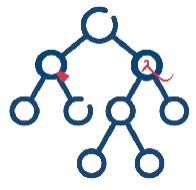
\includegraphics[height=1.0cm]{msca_logo.png}}%
    \end{center}

    \vspace{0.6cm}

    % Main title with Q logos on sides (with clickable links)
    \begin{center}
        \begin{minipage}{0.1\textwidth}
            \centering
            \href{https://quantlet.com}{
\includegraphics[height=1.1cm]{ql_logo.png}}
        \end{minipage}%
        \begin{minipage}{0.78\textwidth}
            \centering
            {\LARGE\bfseries\usebeamercolor[fg]{title}\inserttitle}

            \vspace{0.3cm}

            {\usebeamerfont{subtitle}\usebeamercolor[fg]{title}\insertsubtitle}
        \end{minipage}%
        \begin{minipage}{0.1\textwidth}
            \centering
            \href{https://quantinar.com}{
\includegraphics[height=1.1cm]{qr_logo.png}}
        \end{minipage}
    \end{center}

    \vspace{0.6cm}

    % Authors (left aligned)
    \hspace{0.5cm}{\usebeamerfont{author}\insertauthor}

    \vspace{0.3cm}

    % Institute/Affiliations (left aligned)
    \hspace{0.5cm}\begin{minipage}[t]{0.9\textwidth}
        \raggedright\small\insertinstitute
    \end{minipage}
}

%=============================================================================
% THEOREM ENVIRONMENTS
%=============================================================================
\theoremstyle{definition}
\setbeamertemplate{theorems}[numbered]
\ifdefined\sfmlang
\newtheorem{defn}{Definiție}
\newtheorem{thm}{Teoremă}
\newtheorem{prop}{Propoziție}
\newtheorem{rmk}{Observație}
\else
\newtheorem{defn}{Definition}
\newtheorem{thm}{Theorem}
\newtheorem{prop}{Proposition}
\newtheorem{rmk}{Remark}
\fi

%=============================================================================
% CENTRED MINIPAGE (no extra vertical space)
%=============================================================================
\newenvironment{cminipage}[1]{%
    \par\noindent\hfill\begin{minipage}{#1}\ignorespaces
}{%
    \end{minipage}\hfill\null\par
}

%=============================================================================
% CUSTOM COMMANDS
%=============================================================================
\newcommand{\E}{\mathbb{E}}
\newcommand{\Var}{\text{Var}}
\newcommand{\Cov}{\text{Cov}}
\newcommand{\Corr}{\text{Corr}}
\newcommand{\R}{\mathbb{R}}
\newcommand{\N}{\mathbb{N}}
\newcommand{\Z}{\mathbb{Z}}
\newcommand{\B}{\mathbf{B}}
\newcommand{\imark}{\textcolor{MainBlue}{\textbullet}}
\newcommand{\RMSE}{\text{RMSE}}
\newcommand{\MAE}{\text{MAE}}
\newcommand{\MAPE}{\text{MAPE}}



\newcommand{\qlurl}[1]{https://github.com/danpele/SFM/tree/main/Quantlets/Ch_16/#1}
\renewcommand{\nb}{\colaburl{notebooks/EN/chapter16_seminar_notebook.ipynb}}
\renewcommand{\nbname}{chapter16\_seminar\_notebook.ipynb}
% left column: full width in the student version, narrower next to the solution
\newcommand{\taskw}{\ifsolutions 0.47\textwidth\else 0.96\textwidth\fi}
\newcommand{\solw}{\ifsolutions 0.49\textwidth\else 0pt\fi}

% Clickable citations (DOIs verified via Crossref)

\newcommand{\refFHH}{\href{https://doi.org/10.1007/978-3-030-13751-9}{Franke, Härdle \& Hafner (2019)}}
\newcommand{\refBHL}{\href{https://doi.org/10.1007/978-3-642-33929-5}{Borak, Härdle \& López-Cabrera (2013)}}
\newcommand{\refTsay}{\href{https://doi.org/10.1002/9780470644560}{Tsay (2010)}}
\newcommand{\refCLM}{\href{https://doi.org/10.1515/9781400830213}{Campbell, Lo \& MacKinlay (1997)}}
\newcommand{\refQRM}{\href{https://press.princeton.edu/books/hardcover/9780691166278/quantitative-risk-management}{McNeil, Frey \& Embrechts (2015)}}
\newcommand{\refCont}{\href{https://doi.org/10.1080/713665670}{Cont (2001)}}
\newcommand{\refMandelbrot}{\href{https://doi.org/10.1086/294632}{Mandelbrot (1963)}}
\newcommand{\refNolan}{\href{https://doi.org/10.1007/978-3-030-52915-4}{Nolan (2020)}}
\newcommand{\refJB}{\href{https://doi.org/10.1016/0165-1765(80)90024-5}{Jarque \& Bera (1980)}}
\newcommand{\refHill}{\href{https://doi.org/10.1214/aos/1176343247}{Hill (1975)}}
\newcommand{\refFama}{\href{https://doi.org/10.2307/2325486}{Fama (1970)}}
\newcommand{\refLM}{\href{https://doi.org/10.1093/rfs/1.1.41}{Lo \& MacKinlay (1988)}}
\newcommand{\refEngle}{\href{https://doi.org/10.2307/1912773}{Engle (1982)}}
\newcommand{\refBoll}{\href{https://doi.org/10.1016/0304-4076(86)90063-1}{Bollerslev (1986)}}
\newcommand{\refRM}{\href{https://www.msci.com/documents/10199/5915b101-4206-4ba0-aee2-3449d5c7e95a}{J.P.\ Morgan/Reuters (1996)}}
\newcommand{\refArtzner}{\href{https://doi.org/10.1111/1467-9965.00068}{Artzner et al.\ (1999)}}
\newcommand{\refKupiec}{\href{https://doi.org/10.3905/jod.1995.407942}{Kupiec (1995)}}
\newcommand{\refHurst}{\href{https://doi.org/10.1061/TACEAT.0006518}{Hurst (1951)}}
\newcommand{\refPeters}{\href{https://www.wiley.com/en-us/Fractal+Market+Analysis\%3A+Applying+Chaos+Theory+to+Investment+and+Economics-p-9780471585244}{Peters (1994)}}
\newcommand{\refAltman}{\href{https://doi.org/10.1111/j.1540-6261.1968.tb00843.x}{Altman (1968)}}
\newcommand{\refGKX}{\href{https://doi.org/10.1093/rfs/hhaa009}{Gu, Kelly \& Xiu (2020)}}
\newcommand{\refNakamoto}{\href{https://bitcoin.org/bitcoin.pdf}{Nakamoto (2008)}}
\newcommand{\refAB}{\href{https://doi.org/10.1257/aer.20120555}{Adrian \& Brunnermeier (2016)}}
\newcommand{\refDY}{\href{https://doi.org/10.1016/j.ijforecast.2011.02.006}{Diebold \& Yilmaz (2012)}}
\newcommand{\refMenk}{\href{https://doi.org/10.1111/jofi.13337}{Menkveld et al.\ (2024)}}
\newcommand{\refWang}{\href{https://doi.org/10.1038/s41586-023-06221-2}{Wang et al.\ (2023)}}

\title[Statistics of Financial Markets]{Statistics of Financial Markets}
\subtitle{Seminar 16: Review\ifsolutions\ (instructor version)\fi}
\author[D.T. Pele]{Daniel Traian PELE}
\institute{Bucharest University of Economic Studies\\
IDA Institute Digital Assets\\
Blockchain Research Center\\
AI4EFin Artificial Intelligence for Energy Finance\\
Romanian Academy, Institute for Economic Forecasting\\
MSCA Digital Finance}
\date{}

%=============================================================================
\providecommand{\sfmapplink}[3]{\hypertarget{#2}{}\hyperlink{#1}{\beamergotobutton{#3}}}  % APPLINKS-MACROS
\providecommand{\sfmappback}[2]{\begin{tikzpicture}[remember picture,overlay]\node[anchor=south east] at ([xshift=-3mm,yshift=7mm]current page.south east){\hyperlink{#1}{\beamerreturnbutton{#2}}};\end{tikzpicture}}  % APPLINKS-MACROS
\providecommand{\sfmchlink}[2]{\href{#1}{#2}}  % APPLINKS-MACROS
\providecommand{\sfmchlinkt}[2]{\href{#1}{\usebeamercolor[fg]{frametitle}#2}}  % APPLINKS-MACROS
\begin{document}
%=============================================================================

{
\setbeamertemplate{headline}{}
\setbeamertemplate{footline}{}
\begin{frame}[noframenumbering]
    \titlepage
\end{frame}
}
% BEGIN-ACRONYMS (generat de latex/acronyms.py; nu editati manual)
\begin{frame}{Acronyms used in this material}
\setbeamertemplate{itemize/enumerate body begin}{\tiny}
\begin{columns}[T]
\begin{column}{0.49\textwidth}
\begin{itemize}\setlength{\itemsep}{0pt}
    \item \textbf{AI}: Artificial Intelligence
    \item \textbf{AUC}: Area Under the (ROC) Curve
    \item \textbf{BET}: Bucharest Exchange Trading (index)
    \item \textbf{EAD}: Exposure At Default
    \item \textbf{EODHD}: EOD Historical Data (market-data provider)
    \item \textbf{ES}: Expected Shortfall
    \item \textbf{EWMA}: Exponentially Weighted Moving Average
    \item \textbf{FHS}: Filtered Historical Simulation
    \item \textbf{GARCH}: Generalised AutoRegressive Conditional Heteroskedasticity
    \item \textbf{HS}: Historical Simulation
    \item \textbf{JB}: Jarque–Bera (test)
    \item \textbf{LGD}: Loss Given Default
    \item \textbf{MDD}: Maximum DrawDown
\end{itemize}
\end{column}
\begin{column}{0.49\textwidth}
\begin{itemize}\setlength{\itemsep}{0pt}
    \item \textbf{PD}: Probability of Default
    \item \textbf{SE}: Standard Error
    \item \textbf{SR}: Sharpe Ratio
    \item \textbf{VR}: Variance Ratio
\end{itemize}
\end{column}
\end{columns}
\end{frame}
% END-ACRONYMS

\begin{frame}{Today's Question and Route}
\itemsize{\small}
\begin{itemize}
    \item \textbf{Question}: can you solve, on paper and on data, a problem from any chapter of the course?
    \begin{itemize}
        \item this seminar comes \textbf{before} Lecture 16: the section ``What You Need for Today'' is a formula sheet for all chapters
    \end{itemize}
    \item Route
    \begin{itemize}
        \item Part A: six exam-type problems on paper, from returns to systemic risk
        \item Part B: three data tasks on the BET, the S\&P 500 and Bitcoin, each with an interpretation question
        \item Part C: an AI answer to audit
    \end{itemize}
    \item Notebook for today: \href{\nb}{open the seminar notebook in Google Colab}; each task names its notebook section
    \item The seminar is for practice and is not graded; the solutions of [Proposed] tasks are discussed in class
\end{itemize}
\end{frame}

\begin{frame}{Exercise Map}
\itemsize{\small}
\begin{center}
\footnotesize
\begin{tabular}{>{\raggedright\arraybackslash}p{0.8cm}>{\raggedright\arraybackslash}p{6.6cm}>{\raggedright\arraybackslash}p{1.3cm}>{\raggedright\arraybackslash}p{2.4cm}}
\toprule
\textbf{Task} & \textbf{Topic} & \textbf{Type} & \textbf{Chapters} \\
\midrule
A1 & returns, drawdown, annualisation, Sharpe ratio & Solved & 1 \\
A2 & Jarque--Bera, Student-$t$, Hill, stable scaling & Proposed & 2, 3, 5 \\
A3 & Ljung--Box, variance ratio, robust test & Solved & 7 \\
A4 & GARCH, EWMA and Parkinson volatility & Proposed & 8, 9 \\
A5 & VaR 1\%, ES 2.5\%, Kupiec, traffic light & Proposed & 10 \\
A6 & logit PD, expected loss, AUC, $\Delta$CoVaR & Proposed & 12, 15 \\
B1 & a full check-up of the BET since 2015 & Solved & 1--11 \\
B2 & VaR 1\% backtests: S\&P 500 and Bitcoin & Proposed & 8, 10, 14 \\
B3 & efficiency and memory in two windows & Proposed & 7, 11 \\
C2 & audit an AI answer & Proposed & 0--15 \\
\bottomrule
\end{tabular}
\end{center}
\begin{itemize}
    \item \textbf{[Solved]}: full solution in the slides and in the notebook, a model to follow; \textbf{[Proposed]}: you solve it, following the model
\end{itemize}
\end{frame}

\begin{frame}{Data Used}
\itemsize{\small}
\begin{center}
\footnotesize
\begin{tabular}{llll}
\toprule
\textbf{Series} & \textbf{Source} & \textbf{Price used} & \textbf{Period} \\
\midrule
BET, S\&P 500 & EODHD & close & 2000--2026 \\
Bitcoin & EODHD & close, 7 days a week & 2014--2026 \\
\bottomrule
\end{tabular}
\end{center}
\begin{itemize}
    \item Daily log returns in \%: $r_t = 100\,(\ln P_t - \ln P_{t-1})$, each series on its own calendar; the last day is 18 September 2026
    \item Part A needs only a calculator; Part B uses the notebook, with the functions of the course already written (\texttt{returns}, \texttt{moments}, \texttt{ljung\_box}, \texttt{variance\_ratio}, \texttt{garch\_t}, \texttt{kupiec}, \texttt{hurst\_rs})
\end{itemize}
\end{frame}


%=============================================================================
\section{What You Need for Today}
%=============================================================================

\begin{frame}{What You Need for Today (1/3): Returns, Distributions, Tails}
\itemsize{\small}
{\renewcommand{\arraystretch}{1.3}\begin{center}
\footnotesize
\begin{tabular}{ll}
\toprule
\textbf{Quantity} & \textbf{Formula} \\
\midrule
Returns & $R_t = P_t/P_{t-1} - 1$, \ $r_t = \ln(1 + R_t)$; total: $e^{\sum r_t} - 1$ \\
Annualisation & mean $\times q$, volatility $\times \sqrt{q}$; $q = 252$ (shares), 365 (crypto) \\
Sharpe, drawdown & $(\mu - r_f)/\sigma$, SE $\sqrt{(1 + \mathrm{SR}^2/2)/Y}$; \ $D_t = P_t/\max_{s \le t}P_s - 1$, recovery $d/(1 - d)$ \\
Jarque--Bera & $\frac{n}{6}S^2 + \frac{n}{24}K^2 \sim \chi^2(2)$, \ $\chi^2_{0.95}(2) = 5.99$ \\
Student-$t(\nu)$ & excess kurtosis $6/(\nu - 4)$; unit-variance quantile $t_\nu^{-1}(\alpha)\sqrt{(\nu - 2)/\nu}$ \\
Hill & $\hat\alpha = [\frac1k\sum_{i=1}^k \ln(L_{(i)}/L_{(k+1)})]^{-1}$, SE $\hat\alpha/\sqrt{k}$; moments exist for $p < \alpha$ \\
Stable law & sum of $h$ copies: scale $\times h^{1/\alpha}$ (Normal: $\sqrt{h}$) \\
\bottomrule
\end{tabular}
\end{center}
}
\end{frame}

\begin{frame}{What You Need for Today (2/3): Efficiency, Volatility, Memory}
\itemsize{\small}
{\renewcommand{\arraystretch}{1.3}\begin{center}
\footnotesize
\begin{tabular}{ll}
\toprule
\textbf{Quantity} & \textbf{Formula} \\
\midrule
Ljung--Box & $Q(m) = T(T+2)\sum_{k=1}^m \hat\rho_k^2/(T - k) \sim \chi^2(m)$, \ $\chi^2_{0.95}(4) = 9.49$ \\
Variance ratio & $\mathrm{VR}(q) = 1 + 2\sum_{k=1}^{q-1}(1 - k/q)\hat\rho_k$; \ $Z = (\mathrm{VR} - 1)/\sqrt{2(2q-1)(q-1)/(3qT)}$ \\
Robust VR test & $Z^* = (\mathrm{VR} - 1)/\mathrm{SE}_{rob}$; reject at 5\% if $|Z^*| > 1.96$ \\
EWMA & $\sigma_{t+1}^2 = \lambda\sigma_t^2 + (1 - \lambda)r_t^2$, \ $\lambda = 0.94$ \\
GARCH(1,1) & $\sigma_{t+1}^2 = \omega + \alpha\varepsilon_t^2 + \beta\sigma_t^2$, \ $\bar\sigma^2 = \omega/(1 - \alpha - \beta)$, \ $h_{1/2} = \ln 0.5/\ln(\alpha + \beta)$ \\
GARCH forecast & $E_t\sigma_{t+h}^2 = \bar\sigma^2 + (\alpha + \beta)^{h-1}(\sigma_{t+1}^2 - \bar\sigma^2)$ \\
Parkinson & $\sigma^2 = (\ln H - \ln L)^2/(4\ln 2)$ \\
Hurst & $(R/S)_n \propto n^H$; \ risk over $h$ days $\times h^H$ \\
\bottomrule
\end{tabular}
\end{center}
}
\end{frame}

\begin{frame}{What You Need for Today (3/3): Risk, Backtesting, Credit, Systemic Risk}
\itemsize{\small}
{\renewcommand{\arraystretch}{1.3}\begin{center}
\footnotesize
\begin{tabular}{ll}
\toprule
\textbf{Quantity} & \textbf{Formula} \\
\midrule
VaR, ES & $\mathrm{VaR}_\alpha = -q_\alpha > 0$; \ Normal: $-(\mu + \sigma z_\alpha)$, \ ES $-\mu + \sigma\varphi(z_\alpha)/\alpha$ \\
Values & $z_{0.01} = -2.326$, $z_{0.025} = -1.960$, $\varphi(1.96) = 0.0584$, $t_5^{-1}(0.01) = -3.365$ \\
Kupiec & $LR_{uc} = -2[(n - x)\ln(1 - \alpha) + x\ln\alpha - (n - x)\ln(1 - \hat\pi) - x\ln\hat\pi] \sim \chi^2(1)$, \ $\chi^2_{0.95}(1) = 3.84$ \\
Traffic light (250 days) & green 0--4, yellow 5--9, red 10 or more exceptions \\
Logit, EL & $\mathrm{PD} = 1/(1 + e^{-\eta})$, odds ratio $e^{\beta_j}$; \ EL $=$ PD $\times$ LGD $\times$ EAD \\
AUC, Gini & Gini $= 2\,\mathrm{AUC} - 1$ \\
CoVaR & 1\% quantile regression $X_{sys} = a + bX_i$: CoVaR $= -(a + b\,q_\alpha^i)$, \ $\Delta$CoVaR $= b\,(q_{50}^i - q_\alpha^i)$ \\
\bottomrule
\end{tabular}
\end{center}
}
\end{frame}


%=============================================================================
\section{Part A: Problems on Paper}
%=============================================================================

\begin{frame}{A1: Returns, Drawdown and the Sharpe Ratio [Solved]}
\itemsize{\scriptsize}
\begin{columns}[T]
\begin{column}{0.47\textwidth}
\begin{block}{Task}
\begin{itemize}
    \item A share closes at 50.0, 51.5, 49.8, 52.3, 47.9 and 50.6 RON on six consecutive days.
    \item 1. Compute the five simple and the five log returns, in \%.
    \item 2. Compute the total return from the prices and from $\sum_t r_t$.
    \item 3. Compute the maximum drawdown and the gain needed to return to the peak.
    \item 4. A fund has a daily mean return of 0.04\% and a daily standard deviation of 1.3\%; with $r_f = 3\%$ a year, compute its annual mean, its annual volatility, its Sharpe ratio and the SE of the Sharpe ratio over 10 years.
    \item Report: fourteen numbers and one sentence.
\end{itemize}
\end{block}
\end{column}
\begin{column}{0.49\textwidth}
\begin{exampleblock}{Solution}
\begin{itemize}
    \item 1. $R$: $3.00$, $-3.30$, $5.02$, $-8.41$, $5.64$; $r$: $2.96$, $-3.36$, $4.90$, $-8.79$, $5.48$
    \item 2. $50.6/50 - 1 = 1.20\%$; $\sum r_t = 1.19\%$ and $e^{1.19/100} - 1 = 1.20\%$
    \item 3. MDD $= 47.9/52.3 - 1 = -8.41\%$; gain $52.3/47.9 - 1 = 9.19\%$
    \item 4. $252 \times 0.04 = 10.08\%$; $\sqrt{252} \times 1.3 = 20.64\%$; SR $= (10.08 - 3)/20.64 = 0.343$; SE $= \sqrt{(1 + 0.343^2/2)/10} = 0.33$
    \item Interpretation: the Sharpe ratio is about one SE from zero: ten years of data cannot show that this fund beats the risk-free rate.
\end{itemize}
\end{exampleblock}
\end{column}
\end{columns}
\end{frame}

\begin{frame}{A2: Normality, Tails and Stable Scaling [Proposed]}
\propsub
\itemsize{\scriptsize}
\begin{columns}[T]
\begin{column}{\taskw}
\begin{block}{Task}
\begin{itemize}
    \item $n = 2000$ daily returns: skewness $S = -0.8$, excess kurtosis $K = 9$. The six largest losses, in \%: 11.2, 8.4, 7.7, 6.0, 5.5, 4.9. Model: Seminar 2, A7 and Seminar 5, A1.
    \item 1. Compute JB, its skewness and kurtosis parts, and decide at 5\%.
    \item 2. Compute $\nu$ of a Student-$t$ distribution with the same excess kurtosis.
    \item 3. Compute the Hill estimate $\hat\alpha$ with $k = 5$ and its SE.
    \item 4. A stable law with $\alpha = 1.6$ describes daily returns: compute the 20-day scale factor and compare it with $\sqrt{20}$.
    \item Report: seven numbers, one decision and one sentence.
\end{itemize}
\end{block}
\end{column}
\begin{column}{\solw}
\solonly{%
\begin{exampleblock}{Solution}
\begin{itemize}
    \item 1. $\frac{2000}{6}(0.64) = 213.3$, $\frac{2000}{24}(81) = 6750$, JB $= 6963.3 > 5.99$: normality is rejected
    \item 2. $6/(\nu - 4) = 9 \Rightarrow \nu = 4.67$
    \item 3. logs over 4.9: $0.827$, $0.539$, $0.452$, $0.203$, $0.116$; mean $0.4271$; $\hat\alpha = 2.34$, SE $= 1.05$
    \item 4. $20^{1/1.6} = 6.50$ against $\sqrt{20} = 4.47$
    \item The kurtosis part dominates; with $k = 5$ the Hill estimate is too noisy to decide whether the variance is finite.
\end{itemize}
\end{exampleblock}
}
\end{column}
\end{columns}
\end{frame}

\begin{frame}{A3: Autocorrelation and the Variance Ratio [Solved]}
\itemsize{\scriptsize}
\begin{columns}[T]
\begin{column}{0.47\textwidth}
\begin{block}{Task}
\begin{itemize}
    \item $T = 1500$ daily returns; $\hat\rho_1 = -0.05$, $\hat\rho_2 = 0.03$, $\hat\rho_3 = 0.02$, $\hat\rho_4 = -0.01$; the robust SE of $\widehat{\mathrm{VR}}(5)$ is $0.055$.
    \item 1. Compute the Ljung--Box statistic $Q(4)$ and decide at 5\%.
    \item 2. Compute $\mathrm{VR}(5)$.
    \item 3. Compute $Z(5)$ and $Z^*(5)$ and decide at 5\%.
    \item Report: four numbers, two decisions and one sentence.
\end{itemize}
\end{block}
\end{column}
\begin{column}{0.49\textwidth}
\begin{exampleblock}{Solution}
\begin{itemize}
    \item 1. $\sum\hat\rho_k^2 = 0.0039$; $Q(4) = 5.86 < 9.49$ ($p = 0.210$): not rejected
    \item 2. $1 + 2(-0.040 + 0.018 + 0.008 - 0.002) = 1 + 2 \times (-0.016) = 0.968$
    \item 3. SE $= \sqrt{72/22\,500} = 0.0566$: $Z = -0.57$; $Z^* = (0.968 - 1)/0.055 = -0.58$; both $|Z| < 1.96$: not rejected
    \item Interpretation: no evidence against the random walk at one week; weak-form efficiency is not rejected.
\end{itemize}
\end{exampleblock}
\end{column}
\end{columns}
\end{frame}

\begin{frame}{A4: Volatility Forecasts [Proposed]}
\propsub
\itemsize{\scriptsize}
\begin{columns}[T]
\begin{column}{\taskw}
\begin{block}{Task}
\begin{itemize}
    \item GARCH(1,1), returns in \%: $\omega = 0.05$, $\alpha = 0.10$, $\beta = 0.85$; today $\sigma_t^2 = 2.5$ and $\varepsilon_t = 1.0$. One day of an index: high 105.2, low 101.6. Model: Seminar 9, A1 and A3; Seminar 8, A3 and A5.
    \item 1. Compute $\sigma_{t+1}^2$ and the EWMA forecast with $\lambda = 0.94$.
    \item 2. Compute the persistence, the half-life, the long-run variance and the long-run annual volatility.
    \item 3. Compute $E_t[\sigma_{t+5}^2]$.
    \item 4. Compute the Parkinson variance of the day and the annualised Parkinson volatility.
    \item Report: eight numbers and one sentence.
\end{itemize}
\end{block}
\end{column}
\begin{column}{\solw}
\solonly{%
\begin{exampleblock}{Solution}
\begin{itemize}
    \item 1. $0.05 + 0.10 + 2.125 = 2.275$; EWMA $0.94 \times 2.5 + 0.06 \times 1 = 2.41$
    \item 2. $\alpha + \beta = 0.95$; $h_{1/2} = \ln 0.5/\ln 0.95 = 13.5$ days; $\bar\sigma^2 = 0.05/0.05 = 1.00$; $\sqrt{252} \times 1 = 15.87\%$
    \item 3. $1 + 0.95^4(2.275 - 1) = 1 + 0.8145 \times (2.275 - 1) = 2.038$
    \item 4. $100\ln(105.2/101.6) = 3.482$; $3.482^2/(4\ln 2) = 4.373$; $\sqrt{252 \times 4.373} = 33.2\%$
    \item A calm day lowers the variance, which then moves back to its long-run level of 1; a single wide day says little about annual risk.
\end{itemize}
\end{exampleblock}
}
\end{column}
\end{columns}
\end{frame}

\begin{frame}{A5: VaR, ES and Backtesting [Proposed]}
\propsub
\itemsize{\scriptsize}
\begin{columns}[T]
\begin{column}{\taskw}
\begin{block}{Task}
\begin{itemize}
    \item A position of 2\,000\,000 RON; daily returns with mean 0.05\% and standard deviation 1.2\%. Model: Seminar 10, A1, A3 and A5.
    \item 1. Compute the Normal VaR 1\% and ES 2.5\%, in \% and in RON.
    \item 2. Compute VaR 1\% if the standardised returns are Student-$t$ with $\nu = 5$.
    \item 3. A model has 17 exceptions of VaR 1\% in 1000 days: compute $LR_{uc}$ and decide at 5\%.
    \item 4. Give the Basel zone of 11 exceptions in 250 days.
    \item Report: seven numbers, two decisions and one sentence.
\end{itemize}
\end{block}
\end{column}
\begin{column}{\solw}
\solonly{%
\begin{exampleblock}{Solution}
\begin{itemize}
    \item 1. VaR $= -(0.05 - 2.326 \times 1.2) = 2.74\%$ (54\,832 RON); ES $= -0.05 + 1.2 \times 2.338 = 2.76\%$ (55\,107 RON)
    \item 2. $q = -3.365\sqrt{3/5} = -2.607$; VaR $= -(0.05 + 1.2 \times (-2.607)) = 3.08\%$ (61\,556 RON)
    \item 3. $\ell_0 = -88.17$, $\ell_1 = -86.12$, $LR_{uc} = 4.09 > 3.84$ ($p = 0.043$): rejected; 17 is outside $10 \pm 1.96\sqrt{9.9} = [3.8, 16.2]$
    \item 4. 11 exceptions: red zone (10 or more)
    \item The Student-$t$ tail raises VaR 1\%; a rate of 1.7\% is too high for a VaR 1\% model.
\end{itemize}
\end{exampleblock}
}
\end{column}
\end{columns}
\end{frame}

\begin{frame}{A6: Credit Scoring and CoVaR [Proposed]}
\propsub
\itemsize{\scriptsize}
\begin{columns}[T]
\begin{column}{\taskw}
\begin{block}{Task}
\begin{itemize}
    \item Logit: $\eta = -1.8 + 0.9x_1 - 0.6x_2$, applicant with $x_1 = 1.2$, $x_2 = 2.5$; LGD $= 40\%$, EAD $= 150\,000$ RON. A 1\% quantile regression of the system return on a bank: $a = -1.8$, $b = 0.45$; bank: $q_{0.01} = -6.0\%$, median $0.05\%$. Model: Seminar 12, A1 and A5; Seminar 15, A1.
    \item 1. Compute the PD of the applicant and the odds ratio of $x_1$.
    \item 2. Compute the expected loss of the loan.
    \item 3. A scorecard has Gini $= 0.56$: compute its AUC.
    \item 4. Compute CoVaR 1\% at the bank's VaR and at its median, and $\Delta$CoVaR.
    \item Report: seven numbers and one sentence.
\end{itemize}
\end{block}
\end{column}
\begin{column}{\solw}
\solonly{%
\begin{exampleblock}{Solution}
\begin{itemize}
    \item 1. $\eta = -1.8 + 1.08 - 1.5 = -2.22$; PD $= 1/(1 + e^{2.22}) = 9.80\%$; odds ratio $e^{0.9} = 2.46$
    \item 2. EL $= 9.80\% \times 0.40 \times 150\,000 = 5\,878$ RON
    \item 3. AUC $= (1 + 0.56)/2 = 0.78$
    \item 4. CoVaR $= -(-1.8 + 0.45 \times (-6.0)) = 4.50\%$; median: $1.78\%$; $\Delta$CoVaR $= 0.45 \times 6.05 = 2.72$ pp
    \item A one-unit rise in $x_1$ multiplies the odds of default by 2.46; the distress of the bank raises the VaR of the system by 2.72 percentage points.
\end{itemize}
\end{exampleblock}
}
\end{column}
\end{columns}
\end{frame}


%=============================================================================
\section{Part B: Real Data, Inference and Interpretation}
%=============================================================================

\begin{frame}{B1: A Full Check-Up of the BET [Solved]}
\itemsize{\footnotesize}
\begin{itemize}
\item \textbf{Question}: what do \sfmchlink{https://danpele.github.io/SFM/EN/Courses/chapter1_data_returns_indicators.pdf}{Chapters 1}--\sfmchlink{https://danpele.github.io/SFM/EN/Courses/chapter11_fractal_markets_long_memory.pdf}{11} say about the BET since 2015?
\item \textbf{Inputs}: BET closes since 2 January 2015, daily log returns in \%
\item \textbf{Tasks}
\begin{enumerate}
    \item Compute the annual mean, the volatility, the Sharpe ratio with its SE and the maximum drawdown.
    \item Compute the skewness, the excess kurtosis, JB and the Hill tail index of the losses with $k = 2.5\%$ of $n$.
    \item Compute Ljung--Box $Q(10)$ on $r_t$ and on $r_t^2$, and fit a GARCH(1,1)-$t$.
    \item Compute VaR 1\% and ES 2.5\% by historical simulation and with the Normal distribution.
    \item Interpretation: which three facts would you write in an exam answer about the BET?
\end{enumerate}
\item \textbf{Report}: a table of about fifteen numbers, the chart and three sentences
\item Notebook: section B1
\end{itemize}
\end{frame}

\begin{frame}{B1: Solution [Solved]}
\itemsize{\scriptsize}
\begin{center}
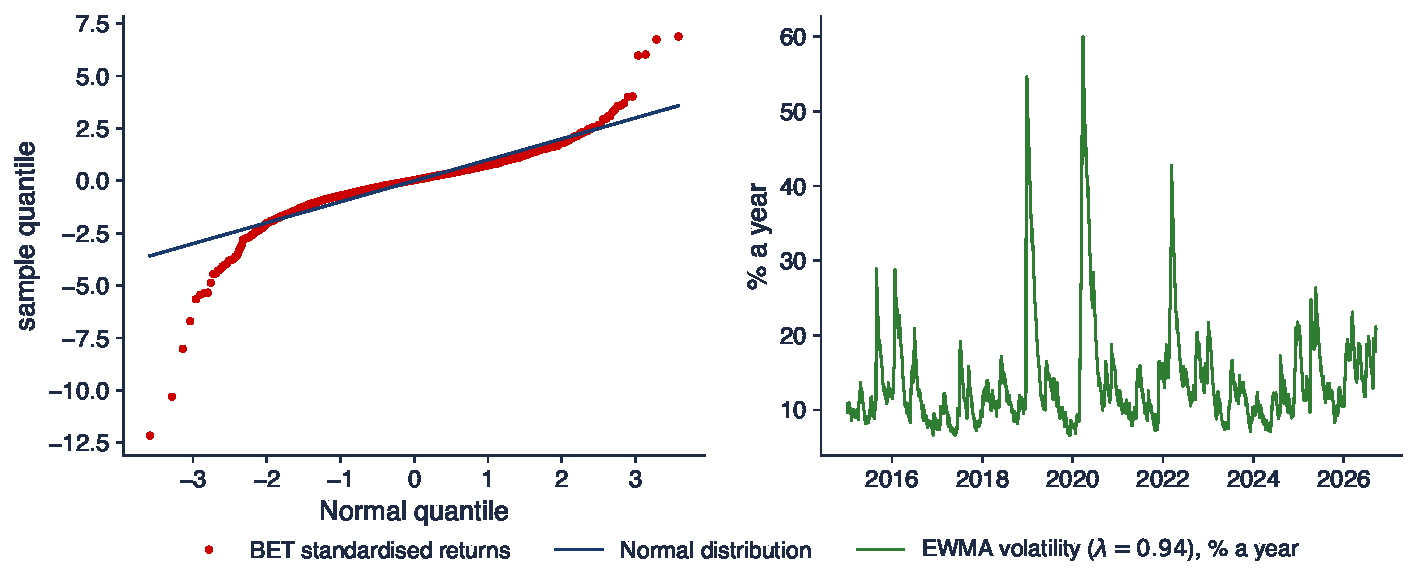
\includegraphics[width=0.96\textwidth,height=0.32\textheight,keepaspectratio]{ch16_sem_b1.pdf}
\end{center}
\vspace{-2mm}
\begin{center}
\scriptsize
\begin{tabular}{llll}
\toprule
\textbf{Performance} & & \textbf{Distribution, dependence} & \\
\midrule
mean, \% a year & $13.2$ & skewness; excess kurtosis & $-1.41$; $17.8$ \\
volatility, \% a year & $15.5$ & JB; Hill $\hat\alpha$ (SE) & 39\,794; $2.19$ ($0.26$) \\
Sharpe (SE) & $0.93$ ($0.35$) & $Q(10)$: $r_t$; $r_t^2$ & $54.7$; $701$ \\
MDD & $-31.1\%$ & GARCH-$t$: $\alpha + \beta$; $h_{1/2}$ & $0.925$; $8.8$ \\
VaR 1\%: HS; Normal & $2.72$; $2.23$ & ES 2.5\%: HS; Normal & $3.21$; $2.24$ \\
\bottomrule
\end{tabular}
\end{center}
\begin{itemize}
    \item $n = 2\,925$, 6 January 2015 -- 18 September 2026; critical value $\chi^2_{0.95}(10) = 18.31$; EWMA volatility peak 60.0\% on 25 March 2020
    \item Interpretation: (1) heavy tails: the Normal VaR 1\% is 18\% too low; (2) returns are weakly autocorrelated, squared returns strongly: volatility clustering; (3) the Sharpe ratio is less than three SE from zero
\end{itemize}\sfmquantlet{Ch_16}{SFM_ch16_seminar}
\end{frame}

\begin{frame}{B2: Backtesting VaR 1\% for the S\&P 500 and Bitcoin [Proposed]}
\itemsize{\footnotesize}
\begin{itemize}
\item \textbf{Question}: does a heavy-tailed method beat a Normal method with fast volatility? Model: B1 and Seminar 10, B3.
\item \textbf{Inputs}: S\&P 500 and Bitcoin, all data; forecasts for every day since 1 January 2017
\item \textbf{Tasks}
\begin{enumerate}
    \item Compute the one-day VaR 1\% by historical simulation on the last 500 returns.
    \item Compute the one-day EWMA-Normal VaR 1\% with $\lambda = 0.94$.
    \item Count the exceptions of each method and run the Kupiec test.
    \item Find the largest number of exceptions in any 250 consecutive days.
    \item Interpretation: which method would a supervisor accept for each series?
\end{enumerate}
\item \textbf{Report}: one table and two sentences
\item Notebook: section B2
\end{itemize}
\end{frame}

\ifsolutions
\begin{frame}{B2: Solution [Proposed]}
\itemsize{\footnotesize}
\begin{center}
\scriptsize
\begin{tabular}{l|rrrr|rrrr}
\toprule
& \multicolumn{4}{c|}{HS (500 days)} & \multicolumn{4}{c}{EWMA-Normal} \\ & exc. & $LR_{uc}$ & $p$ & max 250 & exc. & $LR_{uc}$ & $p$ & max 250 \\
\midrule
S\&P 500 & 29 (1.19\%) & ${0.83}$ & 0.363 & 10 & 57 (2.34\%) & ${31.97}$ & $<$\,0.001 & 13 \\
Bitcoin & 33 (0.93\%) & ${0.18}$ & 0.672 & 6 & 77 (2.17\%) & ${36.78}$ & $<$\,0.001 & 10 \\
\bottomrule
\end{tabular}
\end{center}
\begin{itemize}
    \item Expected exceptions: 24.4 (S\&P 500, 2\,440 days) and 35.5 (Bitcoin, 3\,548 days)
    \item EWMA-Normal has more than twice the target rate on both series: the Normal quantile is too small for heavy tails
    \item HS passes Kupiec, but on the S\&P 500 it has up to 10 exceptions in 250 days (red zone): it reacts slowly
    \item Interpretation: neither is acceptable on its own for the S\&P 500; a model with both a volatility filter and heavy tails (GARCH-$t$, FHS, \sfmchlink{https://danpele.github.io/SFM/EN/Courses/chapter10_var_es_backtesting.pdf}{Chapter 10}) is needed
\end{itemize}\sfmquantlet{Ch_16}{SFM_ch16_seminar}
\end{frame}
\fi

\begin{frame}{B3: Efficiency and Memory in Two Windows [Proposed]}
\itemsize{\footnotesize}
\begin{itemize}
\item \textbf{Question}: did the BET and the S\&P 500 become more efficient after 2015? Model: A3; Seminar 7, B1 and Seminar 11, B1.
\item \textbf{Inputs}: BET and S\&P 500, two windows: 2000--2014 and 2015--2026
\item \textbf{Tasks}
\begin{enumerate}
    \item Compute VR(5) and the robust $Z^*(5)$ in each window.
    \item Compute the Hurst exponent (R/S) of $r_t$ and of $|r_t|$ in each window.
    \item Interpretation: did the BET become more efficient after 2015?
\end{enumerate}
\item \textbf{Report}: one table of sixteen numbers and two sentences
\item Notebook: section B3
\end{itemize}
\end{frame}

\ifsolutions
\begin{frame}{B3: Solution [Proposed]}
\itemsize{\footnotesize}
\begin{center}
\scriptsize
\begin{tabular}{lrrrrrr}
\toprule
& $n$ & VR(5) & $Z^*(5)$ & $p$ & $H$ of $r_t$ & $H$ of $|r_t|$ \\
\midrule
BET, 2000--2014 & 3\,744 & ${1.175}$ & ${2.50}$ & 0.012 & ${0.59}$ & ${0.79}$ \\
BET, 2015--2026 & 2\,925 & ${1.172}$ & ${1.93}$ & 0.054 & ${0.59}$ & ${0.75}$ \\
S\&P 500, 2000--2014 & 3\,770 & ${0.822}$ & ${-2.63}$ & 0.009 & ${0.52}$ & ${0.84}$ \\
S\&P 500, 2015--2026 & 2\,943 & ${0.840}$ & ${-1.34}$ & 0.181 & ${0.53}$ & ${0.84}$ \\
\bottomrule
\end{tabular}
\end{center}
\begin{itemize}
    \item BET: VR(5) above 1 in both windows (momentum); rejected at 5\% before 2015, only borderline after
    \item S\&P 500: VR(5) below 1 (mean reversion), rejected before 2015, not after
    \item $H$ of $|r_t|$ is about 0.75--0.84 in every window: the memory is in the volatility, not in the returns
    \item Interpretation: the BET is closer to weak-form efficiency after 2015, but one test at the 5\% border is weak evidence; rolling windows and Monte Carlo bands would be the next step
\end{itemize}\sfmquantlet{Ch_16}{SFM_ch16_seminar}
\end{frame}
\fi


%=============================================================================
\section{Part C: AI Critique}
%=============================================================================

\begin{frame}{C2: Audit an AI Answer [Proposed]}
\itemsize{\scriptsize}
\begin{itemize}
    \item A student asked an AI assistant to summarise the course for the exam, with the course data. The answer:
    \item \aiprompt{(a) The VaR 99\% of the BET since 2015 is -2.72\%.}
    \item \aiprompt{(b) The BET returns are close to Normal: the skewness is only -1.41.}
    \item \aiprompt{(c) Bitcoin has a daily standard deviation of 3.49\%, so its annual volatility is 55.4\%.}
    \item \aiprompt{(d) For the S\&P 500, alpha + beta = 0.993, so a volatility shock halves in 1/(1 - 0.993) = 139 days.}
    \item \aiprompt{(e) The Hurst exponent of |r| is 0.84 for the S\&P 500, so its returns are predictable and the market is inefficient.}
    \item \aiprompt{(f) For Normal returns, ES 2.5\% and VaR 1\% are almost the same number.}
    \item Tasks
    \begin{itemize}
        \item 1. For each statement, say whether it is correct; if not, give the correct statement and the correct number from the notebook (section C2).
        \item 2. Report: a list of six verdicts with one line of justification each.
    \end{itemize}
\end{itemize}
\end{frame}

\ifsolutions
\begin{frame}{C2: Solution [Proposed]}
\itemsize{\footnotesize}
\begin{itemize}
    \item (a) Wrong twice: the level is the tail probability, VaR 1\%, and VaR is a positive loss: VaR 1\% $= 2.72\%$
    \item (b) Wrong: $S = -1.41$ is far from 0 for daily data, the excess kurtosis is $17.8$ and JB $=$ 39\,794
    \item (c) Wrong: Bitcoin trades 365 days a year: $\sqrt{365} \times 3.49 = 66.6\%$
    \item (d) Wrong: the half-life is $\ln 0.5/\ln 0.993 = 96$ days; $1/(1 - \alpha - \beta)$ is not a half-life
    \item (e) Wrong: memory in $|r_t|$ is memory of the volatility; for $r_t$, $H = 0.53$ and the robust VR test gives $Z^* = -1.34$ (not rejected)
    \item (f) Correct: $\varphi(1.96)/0.025 = 2.338$ against $2.326$, a ratio of 1.005
\end{itemize}\sfmquantlet{Ch_16}{SFM_ch16_seminar}
\end{frame}
\fi


%=============================================================================
\section{Wrap-Up}
%=============================================================================

\begin{frame}{What You Should Take from Today}
\itemsize{\small}
\begin{itemize}
    \item Every exam problem has three parts: the formula with the numbers, the result with its unit and sign, the interpretation
    \item Tests: state $H_0$, the statistic, the critical value, the decision; prefer the robust version
    \item Risk: VaR 1\% is a positive loss; the Normal distribution understates it on real data
    \item Volatility is predictable, the sign of returns almost not
    \item An AI answer is a draft: check the level and the sign of VaR, the annualisation factor and every formula
\end{itemize}
\end{frame}

\begin{frame}{After the Seminar}
\itemsize{\small}
\begin{itemize}
    \item Lecture 16 gathers the course: the course map, one recap slide per chapter, the toolbox, eight solved exam-type problems, the project
    \item Try the [Proposed] tasks on paper first, then check them in the notebook
    \item B3 can grow into a team project: rolling windows, Monte Carlo bands, more emerging markets
    \item Reading: \refFHH; exercises in \refBHL
    \item The seminar is for practice and is not graded; the solutions of [Proposed] tasks are discussed in class
\end{itemize}
\end{frame}


%=============================================================================
\section{References}
%=============================================================================

\begin{frame}{References}
\itemsize{\tiny}
\begin{itemize}
    \item Adrian, T., Brunnermeier, M.K. (2016). \href{https://doi.org/10.1257/aer.20120555}{CoVaR}. \textit{American Economic Review}, 106(7), 1705--1741.
    \item Bollerslev, T. (1986). \href{https://doi.org/10.1016/0304-4076(86)90063-1}{Generalized autoregressive conditional heteroskedasticity}. \textit{Journal of Econometrics}, 31(3), 307--327.
    \item Borak, S., Härdle, W.K., López-Cabrera, B. (2013). \href{https://doi.org/10.1007/978-3-642-33929-5}{\textit{Statistics of Financial Markets: Exercises and Solutions}}, 2nd ed. Springer.
    \item Franke, J., Härdle, W.K., Hafner, C.M. (2019). \href{https://doi.org/10.1007/978-3-030-13751-9}{\textit{Statistics of Financial Markets: An Introduction}}, 5th ed. Springer.
    \item Hill, B.M. (1975). \href{https://doi.org/10.1214/aos/1176343247}{A simple general approach to inference about the tail of a distribution}. \textit{Annals of Statistics}, 3(5), 1163--1174.
    \item Hurst, H.E. (1951). \href{https://doi.org/10.1061/TACEAT.0006518}{Long-term storage capacity of reservoirs}. \textit{Transactions of the American Society of Civil Engineers}, 116(1), 770--799.
    \item Jarque, C.M., Bera, A.K. (1980). \href{https://doi.org/10.1016/0165-1765(80)90024-5}{Efficient tests for normality, homoscedasticity and serial independence of regression residuals}. \textit{Economics Letters}, 6(3), 255--259.
    \item Kupiec, P.H. (1995). \href{https://doi.org/10.3905/jod.1995.407942}{Techniques for verifying the accuracy of risk measurement models}. \textit{Journal of Derivatives}, 3(2), 73--84.
    \item Lo, A.W., MacKinlay, A.C. (1988). \href{https://doi.org/10.1093/rfs/1.1.41}{Stock market prices do not follow random walks: evidence from a simple specification test}. \textit{Review of Financial Studies}, 1(1), 41--66.
\end{itemize}
\end{frame}

\end{document}
